% hydra_satsuma: solver description — certified structure dispatch with a
% satsuma-iter+kissat fall-through.  Build: tectonic doc/hydra_satsuma_solver.tex
% Revised 2026-09-16: third structural stage (multiplier recognition +
% numeric factoring, src/factoring.rs) and its effect on the official-set
% comparison (sec:factoring, sec:factoring-results).
% Revised 2026-10-01: fourth stage (the circuit stage: certified select
% factoring + cut-based re-encoding with DRAT prefixes, src/circuit.rs), the
% hydra_circuit_satsuma arm on the full official set (sec:circuit,
% sec:circuit-results), cactus redrawn with four arms.
\documentclass[10pt]{article}
\usepackage[margin=2.4cm]{geometry}
\usepackage{amsmath,amssymb}
\usepackage{booktabs}
\usepackage{array}
\usepackage{fancyvrb}
\usepackage{enumitem}
\usepackage{microtype}
\usepackage{graphicx}
\usepackage[hidelinks]{hyperref}
\urlstyle{same}
\setlist{itemsep=2pt,topsep=3pt}
\setlength{\emergencystretch}{3em}
\DefineVerbatimEnvironment{Code}{Verbatim}{fontsize=\footnotesize}

\title{\bfseries hydra\_satsuma: Certified Structure Dispatch with a\\
  satsuma-iter+kissat Fall-Through}
\author{Greg Sidebottom}
\date{}

\begin{document}
\maketitle
\vspace{-3em}
\begin{center}
\itshape Research note --- logic repo
(\url{https://github.com/gsidebottom/logic}), SAT track, 2026-08-12;
revised 2026-09-16 with the factoring stage
(\S\ref{sec:factoring}, \S\ref{sec:factoring-results}) and 2026-10-01
with the circuit stage and the \texttt{hydra\_circuit\_satsuma} arm
(\S\ref{sec:circuit}, \S\ref{sec:circuit-results}).
Solver description for the \texttt{hydra\_satsuma} backend of
\texttt{sat}: the certified \texttt{hydra} structure-dispatch pipeline
(Cook-shape prover, factoring stage, XOR/GF(2) stage and, in
\texttt{hydra\_circuit\_satsuma}, a circuit stage) whose fall-through
engine is satsuma-iter+kissat, winner of the SAT Competition 2026 main
track.
Includes the completed apples-to-apples comparison
(\texttt{hydra} / \texttt{satsuma} / \texttt{hydra\_satsuma} /
\texttt{hydra\_circuit\_satsuma}) on the
official 2026 benchmark set, all on one Mac~mini (M4~Pro,
64\,GB; \S\ref{sec:checkercost}).
\end{center}

\section*{Abstract}

\texttt{hydra\_satsuma} is a structure-dispatch SAT solver: before any
CDCL search, it tests the input for algebraic structure that admits a
\emph{polynomial-size certificate}, and only when no structure applies
does it hand the formula to a general-purpose engine. Four structural
stages run in order: (1) a \emph{Cook-shape prover} that recognizes
five cardinality-contradiction families (pigeonhole and its
generalizations) and emits the Cook-1976 extension-variable refutation
as a VeriPB proof --- families on which resolution, and hence any
DRAT-based route without new variables, is exponential; (2) a
\emph{factoring stage} that recognizes a multiplier circuit whose
product is pinned to a number $N$, reads $N$ off the circuit by probing
it, factors $N$ numerically and rebuilds the model by propagation ---
the satisfiable instances of the ezfact and pyhala-braun families in
milliseconds, the model as witness; a number with no fitting factor
pair is recorded but never reported as a verdict, because primality has
no short certificate in any accepted proof system; (3) an
\emph{XOR/GF(2) stage} that recovers parity constraints from their
clausal encodings and runs Gaussian elimination, certifying parity
refutations in VeriPB by Gocht--Nordstr\"om's division-based method
(GN21); (4) in the \texttt{hydra\_circuit\_satsuma} variant, a
\emph{circuit stage} that reads the gates off the clauses and, where a
multiplier's partial products lie hidden in nested multiplexers on the
inputs, recovers them as extension variables and re-encodes the circuit
from cuts of up to six leaves --- each pass emitting a DRAT prefix that
derives its output from its input, so that CaDiCaL's refutation of the
rewritten formula, appended to the prefixes, is a
\texttt{drat-trim}-checked refutation of the original. The fall-through
engine is satsuma-iter+kissat (Anders et al.), the SAT Competition
2026 main-track winner, run unmodified in a container: satsuma
iterates simplify--order--break rounds, adding only unit and binary
breaking clauses, and emits a binary substitution-redundancy (SR)
proof justifying each addition, kissat appends its clausal
refutation to the same file, and \texttt{dsr-trim} verifies the
\emph{composed} proof against the exact CNF handed over --- so
symmetry-broken UNSAT results remain checker-certified. Every
UNSAT path thus produces a machine-checked certificate in a format on
the SAT Competition 2026 checker menu (VeriPB) or in the winner's own
SR chain; SAT results carry the model as witness, projected to the
original variables. On the official 2026 main-track benchmark set,
\texttt{hydra\_satsuma} exceeds the bare winner by a small margin ---
335 vs.\ 334 solved, and PAR-2 2037 vs.\ 2064 under competition
certification scoring --- with the whole margin traceable to the
structural stages. The factoring stage, added after that run, turns the
set's two satisfiable multiplier instances from 30 and 42\,s into
0.07 and 0.20\,s at a measured cost of at most 0.45\,s on any other
instance (7\,s over the whole run); it moves the PAR-2 by $-0.18$ and
leaves the headline unchanged. The circuit stage, run over the whole set
as \texttt{hydra\_circuit\_satsuma} under the same protocol, refutes
two tree multipliers that no arm had reached --- gm16spwtrc in
1{,}789\,s and gm20spctrc in 2{,}308\,s, both certificates checked
after the verdict --- and loses nothing: 337 solved, 196 certified,
PAR-2 2002.

\section{Pipeline}
\label{sec:pipeline}

The backend runs the following stages in order; the first stage to
reach a verdict ends the run. Stage budgets and caps are given with
each stage.

\subsection{Cook-shape prover}
\label{sec:cook}

A syntactic detector (inputs up to $10^6$ clauses) recognizes five
structured UNSAT families, reading the exact clause layout rather than
solving:

\begin{itemize}
\item \textbf{PHP-$n$-$m$} --- the canonical pigeonhole formula,
  $n$ pigeons, $m$ holes, $n > m$;
\item \textbf{RoundRobin} --- sports-scheduling infeasibility,
  a per-pair/per-day two-level pigeonhole;
\item \textbf{Embedded pigeonhole} --- $P$ disjoint at-least-one
  clauses over $S$ complete slot-mutex cliques (a \emph{slot}
  generalizes a hole: a hole for PHP, a day for RoundRobin) with
  $P > S$, the generalization covering e.g.\ MVRoundRobin;
\item \textbf{Clique-coloring} --- a graph asserted to contain a
  $K$-clique yet be $C$-colorable with $K > C$, proved by composing
  the clique-membership and coloring layers;
\item \textbf{Mutilated chessboard} --- bipartite perfect-matching
  infeasibility with imbalanced sides, proved by the two-sided
  cardinality argument.
\end{itemize}

On a match the verdict is UNSAT \emph{by construction}, in
microseconds to milliseconds, and --- when a proof is requested ---
the module emits the corresponding pseudo-Boolean refutation in VeriPB
format. For PHP the proof is exactly Cook's 1976 construction: fresh
variables $Q_{ij} = P_{ij} \lor (P_{im} \land P_{nj})$ encode a
pigeonhole instance with one fewer pigeon and hole; the reduction
iterates down to a trivially refutable base. Each layer is polynomial,
rendered as VeriPB \texttt{red} steps with the definition as witness.
This matters because Haken's 1985 lower bound makes PHP exponential
for resolution: a solver-emitted DRAT proof (which cannot introduce
variables the solver never used) is out of reach at scale, while the
extension-variable route is short, and VeriPB is one of the three
checkers on the SAT Competition 2026 menu
(\S\ref{sec:compliance}). Every detector verifies the clauses its
proof consumes, not only the at-least-one layers: the clique-coloring
detector once accepted the two positive layers alone, and the
unit-propagated residual of a \emph{satisfiable} $6\times 6$
multiplier matched its arity profile (found 2026-09-15 while building
the factoring stage; no competition instance was affected). It now
looks up every mutex its rup steps use, directly or through the
standard encoding's edge variables.

\subsection{Factoring stage}
\label{sec:factoring}

For inputs up to $5\times 10^6$ clauses, the stage tests for a
multiplier circuit $\mathit{out} = a \cdot b$ whose output bits are
pinned by unit clauses to a number $N$ with the factor bits free --- the
shape of the ezfact and pyhala-braun competition families. The structure
is read from the clauses and the encoding conventions from the circuit's
own behaviour:

\begin{itemize}
\item \textbf{Structure.} Parity relations (a 3- or 4-variable set
  carrying every clause of one parity) are the sum cells; union-find
  over their unpinned members gives the product columns. The factor
  bits are the unpinned, relation-free variables that meet at least
  four others in gate clauses (the 4-core of the co-occurrence graph:
  a factor bit meets every bit of the other factor in its
  partial-product gates, a gate output only its few inputs); a
  bipartite split separates the factors and the addition table (which
  pairs meet in which column) labels the bits by weight. Each bit's
  polarity is read off its AND gates, because a shuffled instance flips
  every variable independently.
\item \textbf{Conventions.} 48 random factor assignments are propagated
  through the pin-free CNF. Pins the factor bits never determine and
  that never conflict are the circuit's constants; pins that never
  vary are side constraints (pyhala-braun pins ``the factor is not
  1''); every other pin is matched against the bits of the product
  under the readings of the factor bits --- orientation of the
  labelling and an implicit odd low bit per factor --- and a reading
  that explains the pins fixes $N$. The pyhala-braun labelling comes
  out mirrored; the orientation reading absorbs it.
\item \textbf{Numbers.} Pollard--Brent with Miller--Rabin on $N$;
  every divisor pair of the circuit's widths is tried by propagation
  through the \emph{full} CNF, and the resulting model is checked
  against every clause --- a wrong reading can only miss, never
  mislead.
\end{itemize}

Verdicts: a fitting pair gives SAT with the model as witness
(self-certifying, like the pure-XOR path). A number with no fitting
pair is a \emph{numeric} UNSAT --- reported in the log
(\texttt{factoring-verdict=unsat}) but never as the verdict, because
the primality of $N$ has no short certificate in DRAT, LRAT, SR or
VeriPB; the instance proceeds to the later stages and the engine's
refutation is the certificate. Anything unrecognized falls through at
the structure pass. On the benchmark families the stage reads and
solves ezfact16/32/64 ($N$ the square of a 16- or 32-bit prime, or a
16-bit prime) and pyhala-braun 30/35/40 (satisfiable and
unsatisfiable, $N = 23173\times 23197$, $131101\times 131113$,
$741457\times 741469$); toughsat is not recognized --- its product
bits are folded into the last cells as constants that unit propagation
reads backwards, and the \texttt{toughsat\_}$n$\texttt{bits} encoding is
not an array multiplier at all.

The stage is bounded on every input. Before anything superlinear it
checks plausibility in linear time --- at least eight pins, at most 4096
candidate factor bits, and parity-relation and pin counts consistent
with a multiplier of that many bits (a verification circuit with
thousands of units or hundreds of thousands of candidates is rejected
here) --- and a wall-clock budget of 1\,s
(\texttt{FACTORING\_BUDGET\_MS}) backstops the rest; a multiplier of
competition size is read in well under 200\,ms
(\S\ref{sec:factoring-results}).

\subsection{XOR/GF(2) stage}
\label{sec:xor}

For inputs up to $5\times 10^6$ clauses, the stage recovers XOR
constraints from their CNF encodings (complete canonical encodings
only; the certifier re-derives the recovery strictly, so no trusted
parsing) and runs GF(2) Gaussian elimination. Three outcomes:

\begin{itemize}
\item \textbf{Inconsistent system} (by unit propagation or by GE): the
  formula is UNSAT. When a proof is requested the stage emits a
  parity refutation following Gocht and Nordstr\"om's method
  \cite{gn21} (henceforth \textbf{GN21}): parity reasoning, though
  exponential for resolution, has short pseudo-Boolean certificates,
  because cutting planes' \emph{division} rule captures mod-2
  arithmetic --- encode each recovered XOR as pseudo-Boolean
  constraints, and summing two of them followed by division by two
  derives their GF(2) sum in a constant number of proof steps. Our
  certificate names the (typically small) refuting subset of
  recovered XORs and derives the contradiction $0 \geq 1$ from their
  sum, checkable by \texttt{veripb} in milliseconds. (The certifier
  re-derives the XOR recovery itself from the clausal encodings, so
  the proof does not trust the recovery code.)
\item \textbf{Pure-XOR satisfiable}: GE solves the system outright;
  the model is the certificate.
\item \textbf{Partial simplification}: GE forces some variables and
  simplifies the clause set, yielding an equisatisfiable
  \emph{residual}. What happens next depends on \emph{certified mode}
  (\S\ref{sec:certified}).
\end{itemize}

\subsection{Certified mode}
\label{sec:certified}

The \texttt{--proof} flag is the certified-mode switch for the whole
hydra family. The subtlety is the partial-simplification case: an
engine refutation of the \emph{residual} does not certify the
\emph{original} formula --- the GE step connecting them is real
reasoning that the downstream proof does not contain. Therefore:

\begin{itemize}
\item \textbf{Certified mode} (\texttt{--proof} present; the benchmark
  harness always passes it): the GE simplification is
  \emph{discarded} and the engine solves the original formula. Full
  end-to-end certification beats the simplification --- a trade
  measured to be nearly free (\S\ref{sec:ge-value}).
\item \textbf{Uncertified mode} (no \texttt{--proof}): the engine
  solves the residual. Verdicts remain sound (GE derives only logical
  consequences; SAT models are reconstructed by overwriting GE-forced
  variables), but a residual-path UNSAT is reported explicitly as
  uncertified for the original.
\end{itemize}

Emitting a proof \emph{of the GE step itself} (deriving the forced
units and simplified clauses via extension variables, in DSR or
VeriPB) would close this gap and is well-understood machinery; it is
deliberately deferred because measurement shows nothing is currently
lost (\S\ref{sec:ge-value}).

\subsection{Circuit stage}
\label{sec:circuit}

The \texttt{hydra\_circuit\_satsuma} variant adds a fourth stage
between the structural stages and the fall-through, from the library
module \texttt{logic::circuit} (also the \texttt{cnf2aig} command
line). It is a certified preprocessor for one encoding family, the
GenMul multiplier-verification instances, and it was found by
measurement: on gm16spwtrc --- a 320{,}000-gate decision diagram of
multiplexers, each selected by a primary input --- ABC's \texttt{dc2}
rewriting~\cite{abc,dagaware} in front of CaDiCaL turned a 5000\,s
timeout into an 1{,}872\,s refutation, and what the rewriting did was
recover the partial products, which the CNF spells as two nested
multiplexers on the inputs per product; SAT sweeping, the usual circuit
tool~\cite{kuehlmann02,fraig}, merged 2\% of the gates and changed
nothing. The stage reproduces that effect
natively, with a proof:

\begin{itemize}
\item \textbf{Does it apply?} The gates are read off the clauses
  (AND/OR of any width by pattern, XOR groups, any function of up to
  three inputs by truth table), oriented and ordered with each cycle of
  definitions broken at one gate, and the select factoring below is
  tried without writing anything. The stage applies when factoring finds
  at least 64 products of inputs, put on at least 5\% of the gates and
  shared by at least 20 gates each on average; a hash or an equivalence
  miter has products without sharing and is left alone, and inputs over
  $10^7$ clauses skip the stage. On the official set it fires on 14
  instances (\S\ref{sec:circuit-results}). The trial is bounded by the
  full factoring pass, measured on the 353 official instances under the
  cap: median under a second, 90th percentile 7\,s, maximum 50\,s,
  844\,s in all.
\item \textbf{Probe.} CaDiCaL on the original for 20{,}000 conflicts,
  logging its proof. Array multipliers fall here in a few hundred
  conflicts, and the passes would cost them seconds to minutes; a probe
  verdict is a verdict, CaDiCaL's DRAT its certificate.
\item \textbf{Select factoring.} Where a gate selects between an inner
  multiplexer and that multiplexer's own else-branch,
  $o = s\,?\,(s_2\,?\,a : e) : e$ becomes $o = (s \wedge s_2)\,?\,a : e$.
  The product $s \wedge s_2$ is one extension variable shared by every
  gate that tests the same pair, defined by three clauses that are RAT
  on the new literal; the rewritten gate's clauses are derived from the
  old ones by unit propagation or by cases on the selects, and a gate
  that tests the same variable twice folds. Gates nothing reads any more
  are dropped, their definitions kept aside for model extension. On
  gm16spwtrc: 140{,}523 gates rewritten onto 265 products in 6\,s,
  1.92\,M clauses to 1.08\,M.
\item \textbf{Cut-based re-encoding.} The rewritten circuit is written
  again from cuts of up to six leaves chosen by area flow over four
  rounds: each cut's function, a 64-row truth table evaluated from the
  gates between root and leaves, is covered by its irredundant
  prime-implicant covers (Minato--Morreale~\cite{morreale70,minato93})
  in both polarities, and each resulting clause is derived by cases from
  those gates' definitions; a clause identical to an original one is
  kept rather than re-derived. This is the lean cover ABC's CNF writer
  gives the solver~\cite{een07} --- a multiplexer is four clauses, not
  six, and a cover spans the gates inside a cut --- and it is where most
  of the gain lives: factoring
  alone refutes gm16spwtrc in 3{,}071\,s, factoring then cuts in
  1{,}423\,s.
\item \textbf{Solve and certify.} CaDiCaL (the vendored 3.0.1) takes
  what the passes leave, with the rest of the budget and its own proof.
  Each pass emits a DRAT prefix deriving its output clauses from its
  input and deleting what it replaced; the prefixes concatenate, the
  solver's proof appends, and \texttt{drat-trim} checks the one file
  against the formula the stage was given --- after the verdict, in a
  second bounded phase (\texttt{--circuit-verify-secs}, default the
  solve timeout), exactly as the SR chain's. A SAT model is extended to
  the original variables through the dropped definitions by a CaDiCaL
  call that fixes only the variables of the final formula, and is
  checked against every original clause before it is printed.
\item \textbf{Certified mode.} The stage is handed the original
  formula, never the GE residual of \S\ref{sec:certified}, so its
  certificate covers the input.
\end{itemize}

What the stage is \emph{not}: a general circuit preprocessor. Certified
SAT sweeping --- the fraiging of~\cite{fraig}: simulation-refined
candidate classes, whole cones in a persistent CaDiCaL, the solver's
lemmas as the proof --- is in the same module and was built first; on the unsolved circuits of the set
(gus-md5, slp-aes, sncf, sum\_of\_3\_cubes) neither sweeping nor
ABC's rewriting changes a 5000\,s verdict, and on the multipliers
sweeping adds nothing to factoring. The stage is a hard floor under one
family, with a certificate, and the trigger keeps it off everything
else.

\subsection{Fall-through: satsuma-iter+kissat}
\label{sec:satsuma}

When no structural stage decides the instance, \texttt{hydra\_satsuma}
hands it to the SAT Competition 2026 main-track winner, built
unmodified from the official competition tarball (Anders et al.) and
run in an Ubuntu~24.04 container:

\begin{enumerate}
\item \texttt{satsuma fix <cnf> --bsr --proof-file proof.out --out-file sb.cnf}
  --- the Simplify--Order--Break--Repeat algorithm~\cite{sbr} (Best
  Paper, SAT~2026): iterate \emph{simplify} (CNF preprocessing),
  \emph{order} (clique-guided variable ordering via the
  \textsc{cliquer} maximum-clique solver on the variable--clause
  graph), and \emph{break} (adding \emph{only unit and binary}
  symmetry-breaking clauses, generated systematically along a
  Schreier--Sims pointwise-stabilizer chain), until only trivial
  symmetries remain. Because breaking adds only units and binaries,
  simplification can shrink the formula --- often below the input
  size --- and expose new symmetries for the next round. The emitted
  \emph{binary SR proof} justifies each breaking clause with its
  symmetry as substitution witness;
\item \texttt{kissat sb.cnf proof.out} --- the CDCL engine solves the
  broken formula and \emph{appends} its clausal refutation to the same
  proof file;
\item on UNSAT, \texttt{dsr-trim -f <cnf> proof.out} verifies the
  \emph{composed} proof --- satsuma's SR prefix plus kissat's
  refutation --- against the exact CNF handed over.
\end{enumerate}

The composition is the point: symmetry-breaking clauses are not
consequences of the formula (they are satisfiability-preserving, not
equivalence-preserving), so a bare engine refutation of the broken
formula certifies nothing about the input. SR's substitution witnesses
make the breaking steps checkable, and because kissat's clause
additions are valid SR steps, one checker validates the whole file.
SAT models over satsuma's augmented variable space are projected back
to the original variables (sound: breaking clauses only remove
models).

Operationally the container runs are bounded end to end:

\begin{itemize}
\item \textbf{Solve phase}: in-container \texttt{timeout} at the
  remaining budget minus 2\,s, so the container always self-terminates
  and is never orphaned by the host-side watchdog. The verdict and
  solve time are recorded \emph{before} any verification.
\item \textbf{Verify phase}: a second bounded container run
  (\texttt{--satsuma-verify-secs}, default equal to the solve timeout,
  matching the harness's proof-check budget convention for the LRAT
  chain; $0=$ unlimited). A verification timeout downgrades the row to
  sound-but-unchecked; the verdict is never lost.
\item \textbf{Memory}: optional per-container hard cap
  (\texttt{--satsuma-mem-gb}); an instance exceeding it fails alone.
\item \textbf{Size guard}: instances with $\geq 10^6$ variables or
  $\geq 2.5\times 10^7$ clauses skip satsuma (its literal graph on
  such inputs is several~GB) and run kissat directly on the raw
  formula; an UNSAT proof remains dsr-trim-checkable, since kissat's
  steps are the suffix of every composed proof.
\end{itemize}

The sibling backends complete the family: \texttt{hydra} (same
structural stages, CaDiCaL fall-through with native LRAT checked by
\texttt{cake\_lpr}) and \texttt{satsuma} (the winner bare, no
structural stages --- the baseline arm for measuring what the
dispatch adds).

\section{Certificates by path}
\label{sec:certs}

\begin{center}
\begin{tabular}{@{}llll@{}}
\toprule
Path & Verdict & Certificate & Checker \\
\midrule
Cook shape & UNSAT & Cook-1976 extension proof (VeriPB) & \texttt{veripb} \\
XOR inconsistent & UNSAT & GN21 parity proof (VeriPB) & \texttt{veripb} \\
Pure-XOR solvable & SAT & model witness & --- \\
Multiplier factored & SAT & model witness (propagated from the pair) & --- \\
Multiplier, no factor pair & (none: annotated) & the engine's, below & \\
Circuit stage, probe & UNSAT & CaDiCaL DRAT & \texttt{drat-trim} \\
Circuit stage, passes & UNSAT & DRAT prefixes + CaDiCaL DRAT & \texttt{drat-trim} \\
Circuit stage & SAT & model, extended to the input & --- \\
satsuma+kissat & UNSAT & composed binary SR & \texttt{dsr-trim} \\
satsuma+kissat & SAT & model (projected) & --- \\
GE residual (uncert.\ mode) & UNSAT & none for the original & --- \\
\bottomrule
\end{tabular}
\end{center}

Verification of the SR path happens \emph{in-solver} (the second
container phase), and the harness credits it from the solver's
\texttt{dsr-trim VERIFIED UNSAT} marker rather than re-checking ---
binary SR is not readable by the LRAT/GRAT/VeriPB checkers, and
routing it to one of them would produce a spurious rejection. The
circuit stage's \texttt{drat-trim} check is credited the same way,
from its \texttt{drat-trim VERIFIED UNSAT} marker.

\subsection{Checker cost: hinted vs.\ unhinted}
\label{sec:checkercost}

The two verification chains do structurally different work.
\texttt{cake\_lpr} consumes LRAT, where every step carries
unit-propagation hints computed by CaDiCaL at solve time; checking is
a near-linear replay. \texttt{dsr-trim} consumes unhinted DSR --- like
\texttt{drat-trim}, it must find every propagation itself and
discharge each SR step's redundancy goals, i.e.\ it performs the
elaboration that the LRAT path amortized into the solve. A same-CNF
measurement on the paper's single test platform --- an Apple M4~Pro
Mac~mini (10 performance + 4 efficiency cores), 64\,GB RAM, macOS~26,
the satsuma toolchain in an Ubuntu~24.04 Docker VM; every run in this
note uses it --- (instance \texttt{b20}, ISCAS circuit,
UNSAT):

\begin{center}
\begin{tabular}{@{}lllr@{}}
\toprule
Chain & Proof & Size & Check time \\
\midrule
CaDiCaL native LRAT & hinted & 40\,MB & \texttt{cake\_lpr} 1.55\,s \\
satsuma+kissat DSR & unhinted & 20\,MB & \texttt{dsr-trim} 7.8\,s \\
\bottomrule
\end{tabular}
\end{center}

SR's compensation is succinctness (the same instance's SR proof is
half the LRAT's size; Codel--Avigad--Heule report SR proofs at 0.4\%
of the line count of their RAT translations) and expressiveness (the
symmetry steps have no DRAT analogue without extension variables).
Memory behaves oppositely: \texttt{dsr-trim} is a compact C program
(no out-of-memory events across concurrent checking in our runs),
while \texttt{cake\_lpr}'s CakeML runtime requires a pre-sized heap
that scales with the proof and is the component our harness bounds
with a dedicated memory cap and a concurrency semaphore.

\subsection{Competition-format compliance}
\label{sec:compliance}

SAT Competition 2026 accepts three proof checkers in the main track:
DPR (\texttt{dpr-trim}), GRAT (\texttt{gratgen}), and VeriPB
(\texttt{veripb}). The Cook and GN21 certificates are VeriPB proofs
and verify under the same \texttt{veripb} the competition runs; the SR
chain is the 2026 winner's own; the circuit stage's certificates are
plain DRAT, the RAT fragment of DPR, which \texttt{dpr-trim} reads
unchanged. One gap separates
\texttt{hydra\_satsuma} from literal entry shape: the rules have a
solver declare a \emph{single} checker and write one
\texttt{proof.out}, whereas this backend emits per-path formats.
Unification is mechanical future work --- either translate the
engine's clausal refutations into VeriPB (\texttt{rup}/\texttt{del}
steps map directly; RAT additions become \texttt{red} with witness)
and declare VeriPB for everything, or render the Cook/GN21
constructions in DRAT-with-extension-variables and declare the
clausal chain. The VeriPB route is helped by satsuma itself: its SR
steps can be emitted in either DSR or VeriPB format~\cite{sbr}, so
only the engine refutation needs translating.

\section{Measured design decisions}
\label{sec:ge-value}

Two measurements on the official 2026 main-track set (400 instances
with duplicates; the M4~Pro Mac~mini) fixed design choices in advance of the
full performance run:

\begin{itemize}
\item \textbf{GE simplification is worth $\approx$\,nothing on this
  set.} Every instance on which the partial-simplification path fires
  (twelve, all ISCAS-class circuits) recovers exactly one XOR and
  forces exactly one variable --- on formulas of $2\times 10^3$ to
  $3.4\times 10^5$ variables. Solve-only A/B (original vs.\ residual,
  same engine): \texttt{b20} 7.43\,s vs.\ 7.40\,s, \texttt{s38417}
  1.66\,s vs.\ 1.68\,s, \texttt{c7552} 0.75\,s vs.\ 0.77\,s ---
  within noise. Certified mode's ``ignore GE, solve the original''
  therefore costs nothing measurable, and building the GE-step
  certifier (\S\ref{sec:certified}) is not currently justified by
  performance.
\item \textbf{Where the XOR stage does pay, it is already certified.}
  In the prior full \texttt{hydra} run on this set, eleven instances
  were decided outright by the parity stage in $\sim$10\,ms each, all
  eleven with verified GN21 certificates; twenty-seven more fell to
  the Cook prover with verified VeriPB proofs.
\end{itemize}

\section{The benchmark set: construction and comparability}
\label{sec:benchset}

\subsection{Construction}
\label{sec:benchset-construction}

The evaluation set is the official SAT Competition 2026 main-track
selection, reconstructed as follows and auditable at every step:

\begin{itemize}
\item \textbf{Source of truth}: the competition's
  benchmark-compilation-script tarball
  (\url{https://satcompetition.github.io/2026/downloads/}) carries the
  authoritative \texttt{selected\_benchmarks.csv} with columns
  \texttt{(isohash2, hash, author, family, result)}. The file is
  archived in-repo at
  \path{tools/gbd/sc2026_selected_benchmarks.csv}.
\item \textbf{Slot count and duplicates}: the CSV has exactly
  \textbf{400 rows over 391 distinct hashes}: nine hashes each appear
  twice, \emph{in the official selection itself} (the ISCAS circuit
  \texttt{b20}, hash \texttt{c4318c6a\ldots}, is one of them).
  Re-verified from the archived CSV and from the built index at the
  time of writing.
\item \textbf{Index}: \path{main_track_2026_official.jsonl} is built
  row-for-row from the CSV (400 records), each carrying the hash, the
  original filename, the family/author metadata, and the
  competition's expected result where known.
\item \textbf{Instance identity}: instance files are hash-addressed
  (\texttt{<hash>-<name>.cnf.xz}) and were fetched from the GBD
  benchmark database \emph{by} those hashes; the GBD hash is the MD5
  of the normalized formula (not of the file bytes), so agreement
  between the official CSV and the on-disk files is content-level
  identity under GBD normalization, not filename trust.
\item \textbf{Dedup semantics}: the harness by default deduplicates to
  the 391 unique instances and prints
  \texttt{deduped 9 duplicate records (kept 391 unique)};
  \texttt{--no-dedupe} runs all 400 benchmarks exactly as officially
  scored (a duplicated instance counts twice).
\item \textbf{Result integrity}: every row is cross-checked against
  the competition's expected status where recorded (any
  SAT/UNSAT disagreement is flagged as a mismatch; none has been
  observed), SAT verdicts carry validated witnesses, and UNSAT
  verdicts carry the per-chain certificates of
  \S\ref{sec:certs}.
\end{itemize}

\subsection{Comparability with the official 2026 standings}
\label{sec:benchset-comparability}

Absolute solved counts measured here must \emph{not} be read against
the official competition standings. The official main-track winner,
satsuma-iter+kissat, scored \textbf{276/400} (PAR-2 3647.02) under
5000\,s CPU per instance, one instance per node, on the competition's
cluster hardware. Our protocol runs 5000\,s \emph{wall-clock} per
instance with \emph{ten instances concurrently} on one 14-core Apple
Silicon machine (64\,GB host; the satsuma-based arms execute inside a
$\sim$47\,GB Linux VM). Per-core, per-second compute on the M4~Pro
substantially exceeds the competition nodes'. For reference:

\begin{center}
\begin{tabular}{@{}lrr@{}}
\toprule
Single-thread benchmark & Apple M4 Pro & Xeon Platinum 8368 \\
\midrule
PassMark ST & 4506 & 2345 \\
\bottomrule
\end{tabular}
\end{center}

The local side is the Apple M4~Pro Mac~mini described in
\S\ref{sec:checkercost}. SAT Competition 2026 ran --- for the first
time --- on the NHR@KIT system \emph{HoreKa}, Blue partition, whose
documented nodes are dual Intel Xeon Platinum~8368 (Ice Lake, 2021;
76 cores and $\geq 256$\,GB per node). (An earlier draft assumed the
LMU/SV-COMP cluster from the BenchExec-style Dockerfile in the
winning submission's archive; that Dockerfile pins the benchmarking
\emph{tooling}, not the site.) With 76-core nodes and per-run
CPU-time and memory limits (30\,GB per solver in 2025), many solver
runs share a node --- so \emph{both} environments schedule concurrent
runs against shared memory, ours ten per 14-core machine, theirs
batched per node, and neither side's times are contention-free.
Published single-thread figures put the M4~Pro P-core at roughly
$1.9\times$ the 8368 core (PassMark $4506/2345$); CPU-second vs.\
wall-second accounting differs on top. Equal nominal seconds still
buy substantially more search here, which on heavy-tailed runtimes
pulls many near-timeout instances under the line --- and is why local
solve counts (e.g.\ the \texttt{hydra} baseline's 311 of the 391
unique instances, 318 of the 400 official benchmarks) run well above the
official 276/400. The bare \texttt{satsuma} arm turns this from estimate into
measurement: it is the winner's own pipeline, built unmodified from
the official submission archive, on the official instance set --- so
its local 334/400 against the official 276/400 is a pure environment
delta. Reading it off the cactus curve: local \texttt{satsuma}
reaches 276 solves at a per-instance budget of only \textbf{653\,s},
where the competition needed its full 5000\,s (CPU) for the same
count --- an effective environment factor of
$5000/653 \approx \mathbf{7.7\times}$. This is the all-in
environment difference --- per-core hardware, node scheduling and
contention on both sides, and CPU- vs.\ wall-second accounting fold
into it, and count data alone cannot decompose them. (The estimate is
also count-based, not instance-matched: official per-instance results
are not published alongside the standings.) Notably, the
single-thread microbenchmark ratio above ($\approx 1.9\times$)
\emph{dramatically} underpredicts the measured end-to-end factor:
CDCL search is memory-latency-bound and scheduling-sensitive, and
neither effect is priced by an arithmetic microbenchmark --- a
reminder that microbenchmark constants do not price real workloads.
Local solve counts therefore overshoot official standings
mechanically, by roughly this factor's worth of extra effective
budget per instance. Certification in \S\ref{sec:results} is scored under the
competition's own conditions --- the 45{,}000\,s-per-proof checking
budget ($9\times$ the solve timeout; stated for SC2020 and SC2025,
the standing convention) with ample checker memory --- so no
checking-budget asymmetry remains. The comparisons this note will
report (\S\ref{sec:results}) are therefore \emph{internal}: all four
arms under one fixed protocol on one machine, where hardware and
scheduling effects cancel and only the solver pipelines differ. The
official figures are quoted for context only.

\section{Results}
\label{sec:results}

We report these results \emph{as if the competition were run on an
Apple M4~Pro Mac~mini} (\S\ref{sec:checkercost}), with
the satsuma-toolchain components (satsuma, kissat, \texttt{dsr-trim})
executing under Ubuntu~24.04 in Docker containers. All four arms
completed the official 400-benchmark set at 5000\,s per instance in
certified mode, running ten benchmark processes in parallel
(\texttt{-j 10}) so as to fully utilize the machine's ten
performance cores. Certification is scored under
the competition's conditions: an UNSAT instance counts toward PAR-2
only if its proof verifies within the official 45{,}000\,s checking
budget, with checker memory ample for the chain
(\S\ref{sec:budgetnote}); a check that exceeds the budget leaves the
instance \emph{not solved} for scoring, per the official rule.
Soundness was clean across all four runs: zero expected-status
mismatches, zero witness failures, zero contradictory verdicts
between any pair of arms, and no proof \emph{rejected} by any
checker anywhere in the study.

\begin{center}
\begin{tabular}{@{}lrrrrr@{}}
\toprule
Arm & Solved/400 & SAT & UNSAT & UNSAT certified & PAR-2$^{\ast}$ \\
\midrule
\texttt{hydra} & 318 & 132 & 186 & 185 & 2483 \\
\texttt{satsuma} & 334 & 139 & 195 & 193 & 2064 \\
\texttt{hydra\_satsuma} & 335 & 139 & 196 & 194 & 2037 \\
\texttt{hydra\_circuit\_satsuma} & \textbf{337} & 139 & 198 & \textbf{196} & \textbf{2002} \\
\bottomrule
\end{tabular}

{\footnotesize $^{\ast}$competition scoring: SAT instances and
\emph{certified} UNSAT instances contribute their solve time;
uncertified UNSATs and timeouts contribute $2\times 5000$\,s. The
\texttt{hydra\_satsuma} figure is 2037.35 exactly; with the factoring
stage (\S\ref{sec:factoring-results}, added after this run) it is
2037.17. The \texttt{hydra\_circuit\_satsuma} row (2026-09-30,
\S\ref{sec:circuit-results}) is scored by the same rule, the
official-budget re-check of \S\ref{sec:budgetnote} carried over to
the same instances; the script that scores it reproduces the three
rows above to within 0.2 PAR-2 points.}
\end{center}

All four runs use the identical protocol on all 400 official
benchmarks (the selection's nine duplicate hashes each appear as two
benchmarks and count twice, as in official scoring); the first three
ran in August 2026, the fourth on 2026-09-30.

\begin{figure}[h]
\centering
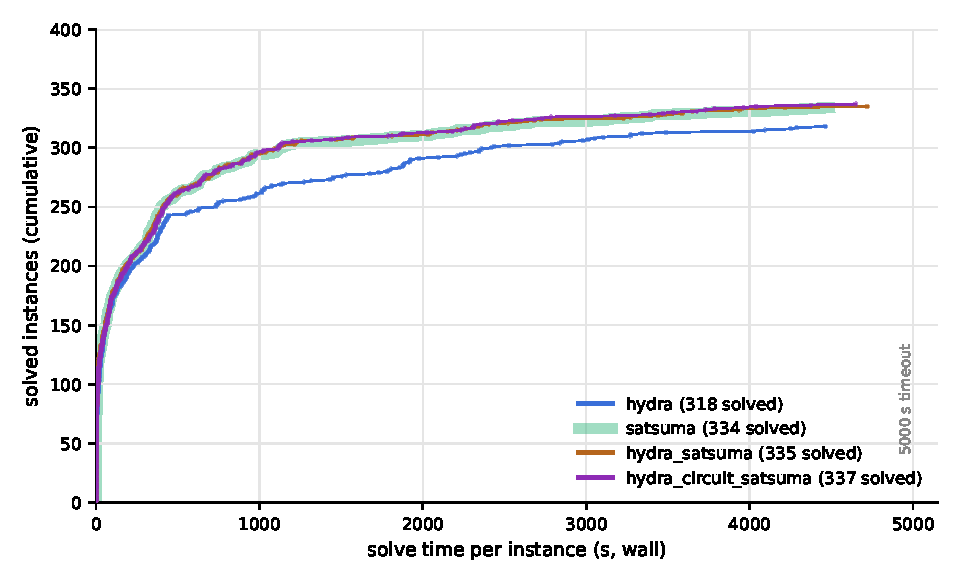
\includegraphics[width=0.86\linewidth]{hydra_satsuma_solver_cactus.pdf}
\caption{Cactus plot on the official 400-benchmark set: cumulative
instances solved within a given per-instance time budget; one dot per
solved instance, every arm aligned to the official benchmarks per
hash. \texttt{satsuma} is drawn as a wide translucent band beneath
\texttt{hydra\_satsuma}'s thin line because the two curves coincide
almost everywhere --- that near-total overlap is itself the finding
(\S\ref{sec:structval}): with a symmetry-capable engine, the
structural front-end changes the curve only at the chessboard pair,
while the engine swap separates both from \texttt{hydra} from
$\sim$250 instances on. \texttt{hydra\_circuit\_satsuma} runs along
\texttt{hydra\_satsuma} and leaves it only at its two multiplier
refutations, 1{,}789 and 2{,}308\,s (\S\ref{sec:circuit-results});
it includes the factoring stage, whose two dots sit under 0.2\,s.}
\label{fig:cactus}
\end{figure}

\textbf{Engine effect} (\texttt{hydra} vs.\ \texttt{hydra\_satsuma},
structure held fixed): replacing CaDiCaL by satsuma-iter+kissat is
worth $+17$ verdicts and, under certification scoring, $-18\%$ PAR-2
($2483 \to 2037$). On the 391 unique instances the satsuma arm solves
eighteen that \texttt{hydra} does not --- concentrated in symmetric
design families (both \texttt{SC25\_Timetable} instances, the
\texttt{lockchart} families, \texttt{ramsey\_4\_4\_18},
\texttt{oddball}, a \texttt{le450} coloring, several
multiplier-equivalence UNSATs) --- against three in the other
direction with no structural signature.

\subsection{What the structural front-end is worth}
\label{sec:structval}

The \texttt{satsuma} vs.\ \texttt{hydra\_satsuma} pair isolates the
Cook/XOR machinery exactly: same engine, same container, same
protocol; the only difference is the structural front-end. Across the
362 benchmarks where no structure applies the two arms' solved sets are
\emph{identical} (zero flips in either direction); every count and
score difference between them traces to the 38 structural benchmarks plus
measurement noise.

\textbf{Benefit where it applies} (38 benchmarks: 27 Cook, 11 GN21):
\texttt{hydra\_satsuma} decides all 38 in \textbf{0.68\,s total},
every verdict carrying a VeriPB certificate that checks in
milliseconds. Bare \texttt{satsuma} solves 37 of 38 at a PAR-2 cost
of 14{,}431\,s: \texttt{mchess\_20} times out (the run's only count
flip), \texttt{mchess\_17} barely lands at 4392.7\,s --- 88\% of
budget, and its SR proof then needs a further 28{,}505\,s of checking
--- and \texttt{tseitingrid6x185\_shuffled}, a Tseitin parity
contradiction, takes 14.1\,s against the GN21 path's 0.025\,s. The
honest fine print: 35 of the 38 are easy for the winner too (median
0.4\,s), so \emph{nearly the whole structural credit concentrates in
the mutilated-chessboard pair} --- the one family in this set that is
resolution-exponential, not rescued by SOBR-style unit/binary
symmetry breaking, and trivial for the two-sided cardinality
argument. The front-end's value against a symmetry-capable engine is
thus a \emph{hard floor under structured families}, plus instant
polynomial certificates, rather than a broad speedup: on a set
without such families it would contribute certification and latency
only; on a set with more of them (larger chessboards, larger Tseitin
grids --- both grow without bound) the count gap widens mechanically.

\textbf{Overhead where it does not apply} (362 benchmarks): measured as the
median paired solve-time difference on the 297 instances both arms
solved --- same formula, same engine, so the pairing isolates the
detection prefix --- the cost is \textbf{$+1.16$\,s per instance},
i.e.\ $\approx 420$\,s over the whole run, or \textbf{1.05 PAR-2
points}. (The paired-difference \emph{sum} is larger, $+3684$\,s, but
the excess beyond the median-based prefix sits in a handful of
multi-thousand-second solves stretching 5--13\% --- proportional to
solve time, the wrong shape for a fixed prefix, and consistent with
wall-clock load variance between runs; kissat's search on identical
input is deterministic.) Detection never caused a flip: no instance
was lost to overhead.

\subsection{The factoring stage on the official set}
\label{sec:factoring-results}

The official set has four prime-factoring benchmarks. Re-run through the
same harness (official index, 5000\,s, \texttt{hydra\_satsuma} with
the stage) on 2026-09-16, against the official \texttt{hydra\_satsuma}
run above:

\begin{center}
\small
\begin{tabular}{@{}lrrp{6.1cm}@{}}
\toprule
Benchmark & official run & with the stage & \\
\midrule
ezfact64\_6 & SAT 30.0\,s & SAT 0.07\,s & factored; witness re-evaluated on all 19{,}785 clauses \\
pyhala-braun-sat-40-4-03 & SAT 42.5\,s & SAT 0.20\,s & factored; witness re-evaluated on all 31{,}795 clauses \\
pyhala-braun-unsat-40-4-02 & UNSAT 43.2\,s & UNSAT 36.9\,s & numeric UNSAT annotated in 0.2\,s; the certificate is kissat's SR proof, \texttt{dsr-trim} verified \\
toughsat\_factoring\_895s & SAT 279.9\,s & SAT 225.8\,s & not recognized; engine path unchanged \\
\bottomrule
\end{tabular}
\end{center}

Only the two satisfiable multiplier instances change hands: they are
decided by the stage in milliseconds, $-72.3$\,s over the run,
$-0.18$ PAR-2 points (2037.35 to 2037.17). The unsatisfiable one
gains nothing real --- the stage knows the answer in 0.2\,s, but the
certificate is still the engine's refutation, so its time is the same
within run-to-run variation, as is toughsat's. Solved counts and
certified counts are unchanged.

\textbf{Cost elsewhere.} The stage is a structure pass on every other
instance, and its cost was measured directly on all 391 unique official
instances rather than inferred from paired runs. The 57 instances above
the $5\times 10^6$-clause cap skip it. On the other 331 (three of them
the recognized multipliers) the median is 0.2\,ms, the 90th percentile
70\,ms and the maximum 0.45\,s (\texttt{q\_query\_3\_L200\_coli},
$3.5\times 10^6$ clauses): 218 are rejected by the pin count before any
superlinear work, and the rest pay the parity-relation pass, linear in
the formula. The total is 7.0\,s over the run --- 0.017 PAR-2 points,
below the resolution of the paired-difference measurement of
\S\ref{sec:structval}. The bounds of \S\ref{sec:factoring} earned
their place: the first, unbounded version of the stage cost 238\,s over
the same set, 44\,s of it on one verification circuit
(\texttt{x-epic\_a19-p16\_step}) whose 427{,}000 candidate bits sent the
candidate filter into a quadratic peel --- the measurement that produced
the plausibility bounds, the incremental peel and the 1\,s budget.

\subsection{The circuit stage on the official set}
\label{sec:circuit-results}

\texttt{hydra\_circuit\_satsuma} ran the official index under the
protocol of \S\ref{sec:results} on 2026-09-30, twenty hours for the
391 unique instances. The stage fires on 14 of them: the twelve GenMul
multiplier-verification instances, \texttt{x-epic\_a10-p53\_transition}
and \texttt{PRP\_40\_40}. On the other 377 it looks and steps aside,
and their verdicts are \texttt{hydra\_satsuma}'s to the instance ---
no flip in either direction, the August run's 65 timeouts reduced to 63
by exactly the two gains below.

\begin{center}
\small
\begin{tabular}{@{}llrrl@{}}
\toprule
Benchmark & \texttt{hydra\_satsuma} & \multicolumn{2}{l}{\texttt{hydra\_circuit\_satsuma}} & certificate \\
\midrule
gm16spwtrc & timeout & UNSAT & 1{,}789\,s & \texttt{drat-trim} 585\,s \\
gm20spctrc & timeout & UNSAT & 2{,}308\,s & \texttt{drat-trim} 197\,s \\
gm16spctrc & UNSAT 511\,s & UNSAT & 60\,s & \texttt{drat-trim} 7\,s \\
gm20sparrc, gm24sparrc, gm28sparrc & UNSAT 0.7--11.5\,s & UNSAT & 0.6--8.1\,s & probe; \texttt{drat-trim} $<$1\,s \\
gm32sparrc, gm36sparrc & UNSAT 5.2--7.6\,s & UNSAT & 6.4--11.2\,s & probe; \texttt{drat-trim} $<$1\,s \\
x-epic\_a10-p53\_transition & UNSAT 9.5\,s & UNSAT & 30.9\,s & \texttt{drat-trim} 174\,s \\
PRP\_40\_40 & SAT 29.2\,s & SAT & 30.7\,s & the model \\
gm16spwtcl, gm24spctbk & timeout & timeout & & \\
gm24spctrc, gm32spctlf & timeout & timeout & & \\
\bottomrule
\end{tabular}
\end{center}

\textbf{Two refutations no arm had reached.} gm16spwtrc and gm20spctrc
are tree multipliers, 16 and 20 bits, where the array multipliers of the
family fall to the probe in a few hundred conflicts; neither the winner's
pipeline nor \texttt{hydra}'s CaDiCaL reaches them in 5000\,s here, at
the $7.7\times$ effective budget of \S\ref{sec:benchset-comparability},
and the competition's selection lists their status as unknown. Both
certificates --- the passes' prefixes followed by CaDiCaL's refutation,
one file --- were accepted by \texttt{drat-trim} against the original
files; under the competition's accounting they are solved instances. A
third, gm16spwtcl, was refuted at 4{,}324\,s in a run of the 14 alone
(\path{doc/competition-benchmark_circuit14_5000_hydra_circuit_satsuma.md})
and timed out in the full run: with ten heavy neighbours the circuit
rows ran 10 to 15\% slower (gm16spwtrc 1{,}549 to 1{,}789\,s,
gm20spctrc 2{,}135 to 2{,}308\,s), enough to carry it over the cliff.
The gain under competition conditions is $+2$, not the targeted run's
$+3$.

\textbf{Where the stage costs.} gm16spctrc, the one tree multiplier
the engine solves, goes from 511 to 60\,s. \texttt{x-epic\_a10-p53} is
the one instance the stage makes slower: the trigger fires, the probe is
undecided, and the passes plus CaDiCaL take 31\,s against satsuma's
9.5\,s, with 174\,s of checking after. \texttt{PRP\_40\_40} is the
stage's one SAT, found by CaDiCaL on the rewritten formula in 31\,s
against the engine's 29\,s, the model extended to the original
variables through the dropped definitions and checked against every
clause. Where the stage does not fire, its trial is the
only cost (\S\ref{sec:circuit}), and no instance was lost to it.

\textbf{Engines.} Of the 337 benchmarks solved: satsuma-iter+kissat
287, the Cook prover 27, GN21 11, the circuit stage 10 (nine UNSAT, one
SAT), the factoring stage 2.

\textbf{Certification.} Every UNSAT the stage claimed checked in-run.
Eighteen satsuma proofs exceeded the harness's 5000\,s check budget ---
the same instances, handed the same CNF, as 18 of \texttt{hydra\_satsuma}'s
25 in August; sixteen of them verified under the official 45{,}000\,s
budget in the re-check of \S\ref{sec:budgetnote}, and the two that did
not are the two proofs uncertifiable in every arm. Hence 196 certified
of 198.

\textbf{Conditions.} On the 206 instances above 20\,s that this run
and the August \texttt{hydra\_satsuma} run both solved outside the
stage, this run is 5\% slower by geometric mean (median 3\%), where
the two August runs differ from each other by 2--3\%. The cause is the
Docker VM: its guest caches the proof files kissat streams through the
bind mount (44\,GB of page cache at one reading), inflating the VM to
its 47\,GB cap, and the host compresses and swaps it. Rows within 10\%
of either 5000\,s cliff should be read as ties; the two gains are not
near one.

\subsection{Certification economics: the proof chains}
\label{sec:budgetnote}

The arms emit certificates through four chains with sharply
different cost profiles; which chains an arm can use is set by its
pipeline. \texttt{hydra} certifies structural verdicts with VeriPB
proofs and engine verdicts with CaDiCaL's native LRAT;
\texttt{satsuma} certifies everything with binary SR;
\texttt{hydra\_satsuma} uses VeriPB for its 38 structural verdicts
and SR for the 158 engine verdicts; \texttt{hydra\_circuit\_satsuma}
adds a fourth chain, plain DRAT checked by \texttt{drat-trim}, for the
circuit stage's nine.

\begin{center}
\begin{tabular}{@{}lllll@{}}
\toprule
Chain & Producer & Checker & Check speed & Check memory \\
\midrule
VeriPB (Cook/GN21) & structural stages & \texttt{veripb} & ms--s & negligible \\
LRAT (hinted) & CaDiCaL & \texttt{cake\_lpr} & s--min & \textbf{the binding axis} \\
SR (unhinted) & satsuma+kissat & \texttt{dsr-trim} & \textbf{the binding axis} & light \\
DRAT (unhinted) & circuit stage + CaDiCaL & \texttt{drat-trim} & s--min & the proof's size \\
\bottomrule
\end{tabular}
\end{center}

\textbf{VeriPB} (38 certificates in each hydra arm): the structural
proofs are polynomial constructions checked in milliseconds to
seconds with negligible memory --- 76 checks across the two arms,
zero at any meaningful cost. When a structural stage fires, its
certificate is effectively free.

\textbf{LRAT + \texttt{cake\_lpr}} (\texttt{hydra}'s 148 engine
certificates): CaDiCaL computes unit-propagation hints during the
solve, so checking is a near-linear replay --- 1.55\,s for a 40\,MB
proof (\texttt{b20}), 58.6\,s for \texttt{stone-width3chain},
62.8\,s for the heaviest verified LRAT in the study. Speed is not
the constraint; \emph{memory} is: \texttt{cake\_lpr}'s CakeML heap
scales with the proof, and of 148 proofs, two needed more than a
16\,GB heap and one (\texttt{hash\_table\_find\_safety\_size\_21})
exceeded even 48\,GB. The checker is formally verified --- the
strongest trust story of the three.

\textbf{SR + \texttt{dsr-trim}} (satsuma-chain certificates: 195 in
\texttt{satsuma}, 158 in \texttt{hydra\_satsuma}): SR proofs are
succinct (half the LRAT's size on the same instance) and can express
symmetry reasoning clausal hints cannot, but they carry no hints, so
the checker performs the propagation search itself --- checking cost
rivals or exceeds solving cost. On the heavy tail, median check time
was 8{,}671\,s with verified checks up to 28{,}505\,s
(\texttt{mchess\_17}); two proofs exceeded the official 45{,}000\,s
budget outright (\texttt{stone-width3chain},
\texttt{hash\_table}). Memory, by contrast, never mattered:
\texttt{dsr-trim} is a compact C program that ran ten-concurrent
without incident throughout.

\textbf{The chains cross.} \texttt{stone-width3chain} is the clean
head-to-head: a $\sim$1-minute solve in every arm, certified by
\texttt{hydra}'s LRAT chain in 58.6\,s while its SR proof is
uncheckable within the official budget --- a $>$750$\times$ gap on
one instance, purely from hints existing. \texttt{hash\_table} is
the double defeat: its SR proof is time-unbounded \emph{and} its
LRAT proof is memory-unbounded (beyond a 48\,GB heap), making it the
one instance in the set uncertifiable under competition conditions
by either engine chain. And \texttt{mchess\_17} completes the
triangle: SR certifies it only after 28{,}505\,s of checking, LRAT
never sees it, and the Cook prover certifies it in a millisecond ---
on structured instances, the structural chain dominates both engine
chains on every axis at once.

\textbf{Reading.} The comparison resolves cleanly. The engine is worth
$+16$/$+17$ verdicts over CaDiCaL on this set; the structural
front-end is worth $+1$ verdict, $+1$ certified instance, and 27
PAR-2 points against the strongest available engine --- at a measured
cost of $\approx 1$ PAR-2 point of detection prefix and zero lost
instances; the factoring stage adds two millisecond solves where the
engine needed 30--42\,s, for a prefix of at most 0.45\,s (7\,s over
the run); the circuit stage adds two certified refutations no arm had
reached and 35 PAR-2 points, on the one family it is built for, for a
trial of at most 50\,s on any instance and no instance lost. Its
deeper contributions are invariants the count does not show: instant polynomial certificates on structured families
(against engine-time SR proofs that are expensive to check --- and
on this set twice uncheckable even at the official budget), and a
hard floor that is unbounded in the direction the engine's weakness
grows.

\section*{Acknowledgments}

Claude (Fable 5, Anthropic) assisted with the implementation,
measurement, and drafting throughout. satsuma and dejavu are by
Markus Anders et al.; kissat by Armin Biere; \texttt{dsr-trim} and
\texttt{lsr-check} by Cayden Codel; \texttt{cake\_lpr} by Yong Kiam
Tan, Marijn Heule, and Magnus Myreen; VeriPB by Stephan Gocht, Jakob
Nordstr\"om, et al. The satsuma-iter+kissat components are built
unmodified from the official SAT Competition 2026 submission archive
and run as-is in a container.

\begin{thebibliography}{99}
\setlength{\itemsep}{2pt}

\bibitem{cook71} S.~A. Cook.
\newblock The complexity of theorem-proving procedures.
\newblock \emph{STOC}, 1971.

\bibitem{cook76} S.~A. Cook.
\newblock A short proof of the pigeon hole principle using extended
  resolution.
\newblock \emph{SIGACT News}, 8(4):28--32, 1976.

\bibitem{haken85} A.~Haken.
\newblock The intractability of resolution.
\newblock \emph{Theoretical Computer Science}, 39:297--308, 1985.

\bibitem{gn21} S.~Gocht and J.~Nordstr\"om.
\newblock Certifying parity reasoning efficiently using pseudo-Boolean
  proofs.
\newblock \emph{AAAI}, 2021.

\bibitem{srcheck} C.~R. Codel, J.~Avigad, and M.~J.~H. Heule.
\newblock Verified substitution redundancy checking.
\newblock \emph{FMCAD}, 2024.
\newblock \url{https://www.cs.cmu.edu/~mheule/publications/SRcheck.pdf}

\bibitem{cakelpr} Y.~K. Tan, M.~J.~H. Heule, and M.~O. Myreen.
\newblock \texttt{cake\_lpr}: Verified propagation redundancy checking
  in CakeML.
\newblock \emph{TACAS}, 2021.

\bibitem{lratfaster} F.~Pollitt, M.~Fleury, and A.~Biere.
\newblock Faster LRAT checking than solving with CaDiCaL.
\newblock \emph{SAT}, 2023.

\bibitem{satcomp26} SAT Competition 2026: certificates and checkers.
\newblock \url{https://satcompetition.github.io/2026/output.html};
  winner submission archive
  \url{https://satcompetition.github.io/2026/downloads/solvers/anders.tar.xz}.

\bibitem{kuehlmann02} A.~Kuehlmann, V.~Paruthi, F.~Krohm, and M.~K. Ganai.
\newblock Robust Boolean reasoning for equivalence checking and
  functional property verification.
\newblock \emph{IEEE Trans.\ CAD}, 21(12):1377--1394, 2002.

\bibitem{fraig} A.~Mishchenko, S.~Chatterjee, R.~Jiang, and R.~Brayton.
\newblock FRAIGs: A unifying representation for logic synthesis and
  verification.
\newblock ERL Technical Report, EECS Dept., UC Berkeley, March 2005.

\bibitem{dagaware} A.~Mishchenko, S.~Chatterjee, and R.~Brayton.
\newblock DAG-aware AIG rewriting: A fresh look at combinational logic
  synthesis.
\newblock \emph{DAC}, 2006.

\bibitem{abc} R.~Brayton and A.~Mishchenko.
\newblock ABC: An academic industrial-strength verification tool.
\newblock \emph{CAV}, LNCS 6174, pp.~24--40, 2010.
\newblock \url{https://github.com/berkeley-abc/abc}

\bibitem{een07} N.~Een, A.~Mishchenko, and N.~S\"orensson.
\newblock Applying logic synthesis for speeding up SAT.
\newblock \emph{SAT}, LNCS 4501, pp.~272--286, 2007.

\bibitem{morreale70} E.~Morreale.
\newblock Recursive operators for prime implicant and irredundant normal
  form determination.
\newblock \emph{IEEE Trans.\ Computers}, C-19(6):504--509, 1970.

\bibitem{minato93} S.~Minato.
\newblock Fast generation of prime-irredundant covers from binary
  decision diagrams.
\newblock \emph{IEICE Trans.\ Fundamentals}, E76-A(6):967--973, 1993.

\bibitem{sbr} M.~Anders, C.~Codel, and M.~J.~H. Heule.
\newblock Simplify, order, break, repeat.
\newblock \emph{SAT 2026}, LIPIcs vol.~377, article~4, pp.~4:1--4:19.
\newblock DOI \path{10.4230/LIPIcs.SAT.2026.4}. Best Paper Award,
  SAT~2026. Software: DOI \path{10.5281/zenodo.20185023}; satsuma:
  \url{https://github.com/markusa4/satsuma}.

\end{thebibliography}

\end{document}
